\documentclass{report}
% Include all project wide packages here.
\usepackage{fullpage}
\usepackage[style=ieee]{biblatex}
\usepackage[dutch]{babel}

\renewcommand{\familydefault}{\sfdefault}

\setmainfont[Ligatures=TeX]{Myriad Pro}
\setmathfont{Asana Math}
\setmonofont{Lucida Console}

\usepackage{titlesec, blindtext, color}
\definecolor{gray75}{gray}{0.75}
\newcommand{\hsp}{\hspace{20pt}}
\titleformat{\chapter}[hang]{\Huge\bfseries}{\thechapter\hsp\textcolor{gray75}{|}\hsp}{0pt}{\Huge\bfseries}
\renewcommand{\familydefault}{\sfdefault}
\renewcommand{\arraystretch}{1.2}
\setlength\parindent{0pt}

%For code listings
\definecolor{black}{rgb}{0,0,0}
\definecolor{browntags}{rgb}{0.65,0.1,0.1}
\definecolor{bluestrings}{rgb}{0,0,1}
\definecolor{graycomments}{rgb}{0.4,0.4,0.4}
\definecolor{redkeywords}{rgb}{1,0,0}
\definecolor{bluekeywords}{rgb}{0.13,0.13,0.8}
\definecolor{greencomments}{rgb}{0,0.5,0}
\definecolor{redstrings}{rgb}{0.9,0,0}
\definecolor{purpleidentifiers}{rgb}{0.01,0,0.01}


\lstdefinestyle{csharp}{
language=[Sharp]C,
showspaces=false,
showtabs=false,
breaklines=true,
showstringspaces=false,
breakatwhitespace=true,
escapeinside={(*@}{@*)},
columns=fullflexible,
commentstyle=\color{greencomments},
keywordstyle=\color{bluekeywords}\bfseries,
stringstyle=\color{redstrings},
identifierstyle=\color{purpleidentifiers},
basicstyle=\ttfamily\small}

\lstdefinestyle{c}{
language=C,
showspaces=false,
showtabs=false,
breaklines=true,
showstringspaces=false,
breakatwhitespace=true,
escapeinside={(*@}{@*)},
columns=fullflexible,
commentstyle=\color{greencomments},
keywordstyle=\color{bluekeywords}\bfseries,
stringstyle=\color{bluestrings},
identifierstyle=\color{purpleidentifiers}
}

\lstdefinestyle{vhdl}{
language=VHDL,
showspaces=false,
showtabs=false,
breaklines=true,
showstringspaces=false,
breakatwhitespace=true,
escapeinside={(*@}{@*)},
columns=fullflexible,
commentstyle=\color{greencomments},
keywordstyle=\color{bluekeywords}\bfseries,
stringstyle=\color{redstrings},
identifierstyle=\color{purpleidentifiers}
}

\lstdefinestyle{xaml}{
language=XML,
showspaces=false,
showtabs=false,
breaklines=true,
showstringspaces=false,
breakatwhitespace=true,
escapeinside={(*@}{@*)},
columns=fullflexible,
commentstyle=\color{greencomments},
keywordstyle=\color{redkeywords},
stringstyle=\color{bluestrings},
tagstyle=\color{browntags},
morestring=[b]",
  morecomment=[s]{<?}{?>},
  morekeywords={xmlns,version,typex:AsyncRecords,x:Arguments,x:Boolean,x:Byte,x:Char,x:Class,x:ClassAttributes,x:ClassModifier,x:Code,x:ConnectionId,x:Decimal,x:Double,x:FactoryMethod,x:FieldModifier,x:Int16,x:Int32,x:Int64,x:Key,x:Members,x:Name,x:Object,x:Property,x:Shared,x:Single,x:String,x:Subclass,x:SynchronousMode,x:TimeSpan,x:TypeArguments,x:Uid,x:Uri,x:XData,Grid.Column,Grid.ColumnSpan,Click,ClipToBounds,Content,DropDownOpened,FontSize,Foreground,Header,Height,HorizontalAlignment,HorizontalContentAlignment,IsCancel,IsDefault,IsEnabled,IsSelected,Margin,MinHeight,MinWidth,Padding,SnapsToDevicePixels,Target,TextWrapping,Title,VerticalAlignment,VerticalContentAlignment,Width,WindowStartupLocation,Binding,Mode,OneWay,xmlns:x}
}

%defaults
\lstset{
basicstyle=\ttfamily\small,
extendedchars=false,
numbers=left,
numberstyle=\ttfamily\tiny,
stepnumber=1,
tabsize=4,
numbersep=5pt
}

\title{Meetrapport: Opamps - Werking \& Afleiding}
\author{Robin Hes\\\&\\Erwin R. de Haan}

\begin{document}
\chapter{Werking \& Afleiding}

\section{Theorie}
Een relaxatie-oscillator maakt het, zoals al gezegd, mogelijk om een analoog signaal op een manier te coderen die bruikbaar is voor digitale systemen. Dit betekent dat een bepaald spanningsniveau moet worden omgezet naar een reeks ``enen en nullen'' of equivalenten daarvan die door het digitale systeem zijn te onderscheiden als twee verschillende waarden. Een relaxatie-oscillator bereikt dit doel door het analoge signaal om te zetten naar een bloksignaal met een periode die afhankelijk is van de waarde van het ingangssignaal.

\begin{figure}[H]
	\centering
	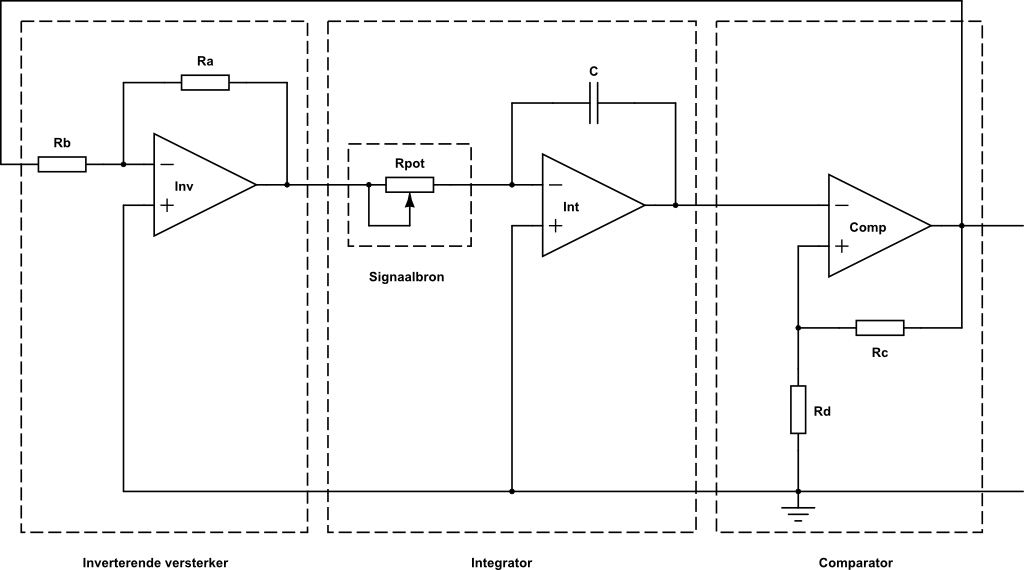
\includegraphics[width=0.8\textwidth]{relaxatie-oscillator.png}
	\caption{De relaxatie-oscillator}
	\label{fig:rel-os}
\end{figure}

Zoals te zien in figuur \ref{fig:rel-os} bestaat de relaxatie-oscillator uit drie afzonderlijke onderdelen: een integrator, een comparator en een inverterende versterker, allen gebaseerd op een op-amp met terugkoppelcircuit. We zullen hieronder per onderdeel een beschrijving geven van de functie in het geheel.

\subsection{Integrator}

De eerste stap in het digitaliseren van het ingangssignaal is om het signaal te integreren. Het signaal is op een punt in de tijd constant, waardoor integratie een lineaire functie oplevert. Als we een blokgolf zouden invoeren, betekent dit dat de integrator een driehoekige functie oplevert, bij de overgang van hoog naar laag levert integratie een dalende lineaire functie op, bij de overgang van laag naar hoog is deze stijgend.\\

\begin{wrapfigure}{r}{0.5\textwidth}
	\centering
	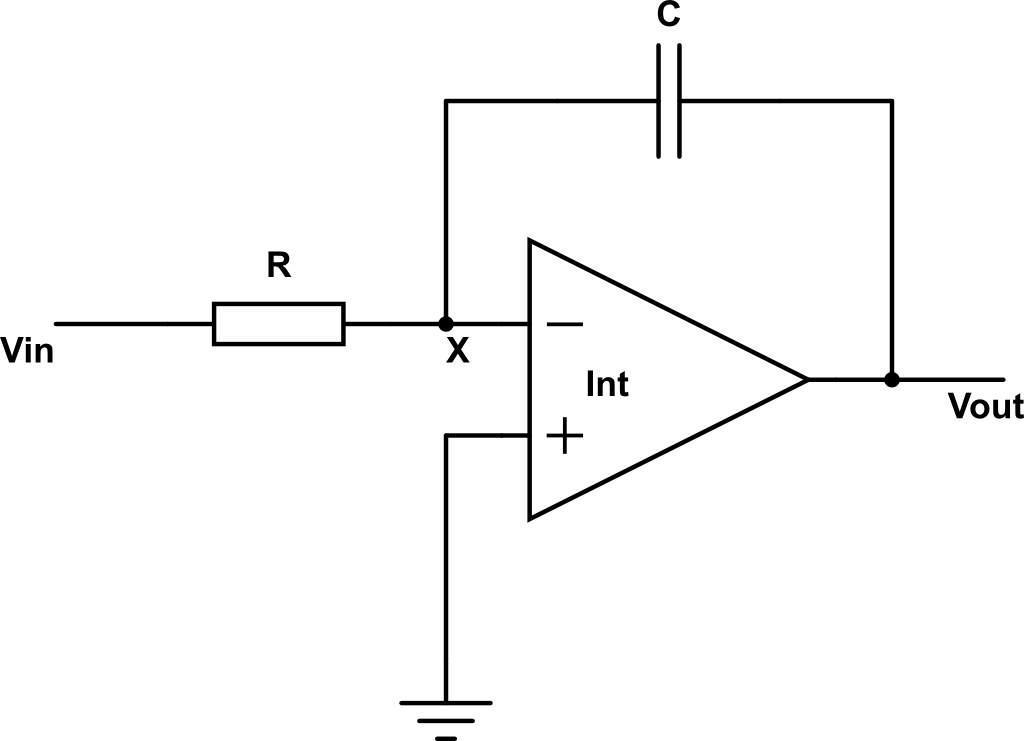
\includegraphics[width=0.4\textwidth]{integrator.png}
	\caption{De relaxatie-oscillator}
	\label{fig:int}
\end{wrapfigure}

De integrator, zoals weergegeven in figuur \ref{fig:int}, zou gezien kunnen worden als een inverterende spanningsversterker met een capaciteit in het terugkoppelcircuit, in plaats van een weerstand. Om de uitgangsspanning te berekenen als functie van de ingangsspanning stellen we een knooppuntsvergelijking op in knooppunt $X$.

$$\frac{V_{X} - V{in}}{R} + V_{X} \cdot j\omega C = 0$$

\noindent
Omdat voor de op-amp de nul-conditie geldt dat $V_{+} = V_{X} = V_{-} = 0$ volgt:

$$-\frac{V_{in}}{R} - V_{out} \cdot j\omega C = 0$$

\noindent
En dus, omdat de stroom door een capaciteit evenredig is met de afgeleide van de spanning over de tijd:

\begin{equation}
	V_{out} = -\frac{V_{in}}{j\omega CR} = -\int_0^t \frac{V_{in}}{RC} \mathrm{d}t
	\label{eq:integrator}
\end{equation}

\noindent
Het door de integrator geleverde signaal voeren we vervolgens in de comparator, het volgende onderdeel.

\subsection{Comparator}


\end{document}